\documentclass[11pt,preprint, authoryear]{elsarticle}

\usepackage{lmodern}
%%%% My spacing
\usepackage{setspace}
\setstretch{1.2}
\DeclareMathSizes{12}{14}{10}{10}

% Wrap around which gives all figures included the [H] command, or places it "here". This can be tedious to code in Rmarkdown.
\usepackage{float}
\let\origfigure\figure
\let\endorigfigure\endfigure
\renewenvironment{figure}[1][2] {
    \expandafter\origfigure\expandafter[H]
} {
    \endorigfigure
}

\let\origtable\table
\let\endorigtable\endtable
\renewenvironment{table}[1][2] {
    \expandafter\origtable\expandafter[H]
} {
    \endorigtable
}


\usepackage{ifxetex,ifluatex}
\usepackage{fixltx2e} % provides \textsubscript
\ifnum 0\ifxetex 1\fi\ifluatex 1\fi=0 % if pdftex
  \usepackage[T1]{fontenc}
  \usepackage[utf8]{inputenc}
\else % if luatex or xelatex
  \ifxetex
    \usepackage{mathspec}
    \usepackage{xltxtra,xunicode}
  \else
    \usepackage{fontspec}
  \fi
  \defaultfontfeatures{Mapping=tex-text,Scale=MatchLowercase}
  \newcommand{\euro}{€}
\fi

\usepackage{amssymb, amsmath, amsthm, amsfonts}

\def\bibsection{\section*{References}} %%% Make "References" appear before bibliography


\usepackage[round]{natbib}

\usepackage{longtable}
\usepackage[margin=2.3cm,bottom=2cm,top=2.5cm, includefoot]{geometry}
\usepackage{fancyhdr}
\usepackage[bottom, hang, flushmargin]{footmisc}
\usepackage{graphicx}
\numberwithin{equation}{section}
\numberwithin{figure}{section}
\numberwithin{table}{section}
\setlength{\parindent}{0cm}
\setlength{\parskip}{1.3ex plus 0.5ex minus 0.3ex}
\usepackage{textcomp}
\renewcommand{\headrulewidth}{0.2pt}
\renewcommand{\footrulewidth}{0.3pt}

\usepackage{array}
\newcolumntype{x}[1]{>{\centering\arraybackslash\hspace{0pt}}p{#1}}

%%%%  Remove the "preprint submitted to" part. Don't worry about this either, it just looks better without it:
\makeatletter
\def\ps@pprintTitle{%
  \let\@oddhead\@empty
  \let\@evenhead\@empty
  \let\@oddfoot\@empty
  \let\@evenfoot\@oddfoot
}
\makeatother

 \def\tightlist{} % This allows for subbullets!

\usepackage{hyperref}
\hypersetup{breaklinks=true,
            bookmarks=true,
            colorlinks=true,
            citecolor=blue,
            urlcolor=blue,
            linkcolor=blue,
            pdfborder={0 0 0}}


% The following packages allow huxtable to work:
\usepackage{siunitx}
\usepackage{multirow}
\usepackage{hhline}
\usepackage{calc}
\usepackage{tabularx}
\usepackage{booktabs}
\usepackage{caption}


\newenvironment{columns}[1][]{}{}

\newenvironment{column}[1]{\begin{minipage}{#1}\ignorespaces}{%
\end{minipage}
\ifhmode\unskip\fi
\aftergroup\useignorespacesandallpars}

\def\useignorespacesandallpars#1\ignorespaces\fi{%
#1\fi\ignorespacesandallpars}

\makeatletter
\def\ignorespacesandallpars{%
  \@ifnextchar\par
    {\expandafter\ignorespacesandallpars\@gobble}%
    {}%
}
\makeatother

\newlength{\cslhangindent}
\setlength{\cslhangindent}{1.5em}
\newenvironment{CSLReferences}%
  {\setlength{\parindent}{0pt}%
  \everypar{\setlength{\hangindent}{\cslhangindent}}\ignorespaces}%
  {\par}


\urlstyle{same}  % don't use monospace font for urls
\setlength{\parindent}{0pt}
\setlength{\parskip}{6pt plus 2pt minus 1pt}
\setlength{\emergencystretch}{3em}  % prevent overfull lines
\setcounter{secnumdepth}{5}

%%% Use protect on footnotes to avoid problems with footnotes in titles
\let\rmarkdownfootnote\footnote%
\def\footnote{\protect\rmarkdownfootnote}
\IfFileExists{upquote.sty}{\usepackage{upquote}}{}

%%% Include extra packages specified by user
\usepackage{booktabs}
\usepackage{longtable}
\usepackage{array}
\usepackage{multirow}
\usepackage{wrapfig}
\usepackage{float}
\usepackage{colortbl}
\usepackage{pdflscape}
\usepackage{tabu}
\usepackage{threeparttable}
\usepackage{threeparttablex}
\usepackage[normalem]{ulem}
\usepackage{makecell}
\usepackage{xcolor}

%%% Hard setting column skips for reports - this ensures greater consistency and control over the length settings in the document.
%% page layout
%% paragraphs
\setlength{\baselineskip}{12pt plus 0pt minus 0pt}
\setlength{\parskip}{12pt plus 0pt minus 0pt}
\setlength{\parindent}{0pt plus 0pt minus 0pt}
%% floats
\setlength{\floatsep}{12pt plus 0 pt minus 0pt}
\setlength{\textfloatsep}{20pt plus 0pt minus 0pt}
\setlength{\intextsep}{14pt plus 0pt minus 0pt}
\setlength{\dbltextfloatsep}{20pt plus 0pt minus 0pt}
\setlength{\dblfloatsep}{14pt plus 0pt minus 0pt}
%% maths
\setlength{\abovedisplayskip}{12pt plus 0pt minus 0pt}
\setlength{\belowdisplayskip}{12pt plus 0pt minus 0pt}
%% lists
\setlength{\topsep}{10pt plus 0pt minus 0pt}
\setlength{\partopsep}{3pt plus 0pt minus 0pt}
\setlength{\itemsep}{5pt plus 0pt minus 0pt}
\setlength{\labelsep}{8mm plus 0mm minus 0mm}
\setlength{\parsep}{\the\parskip}
\setlength{\listparindent}{\the\parindent}
%% verbatim
\setlength{\fboxsep}{5pt plus 0pt minus 0pt}



\begin{document}



\begin{frontmatter}  %

\title{Yield Spreads}

% Set to FALSE if wanting to remove title (for submission)




\author[Add1]{Sven Wellmann}
\ead{20850980@sun.ac.za}





\address[Add1]{Stellenbosch University, Stellenbosch, South Africa}



\vspace{1cm}





\vspace{0.5cm}

\end{frontmatter}



%________________________
% Header and Footers
%%%%%%%%%%%%%%%%%%%%%%%%%%%%%%%%%
\pagestyle{fancy}
\chead{}
\rhead{}
\lfoot{}
\rfoot{\footnotesize Page \thepage}
\lhead{}
%\rfoot{\footnotesize Page \thepage } % "e.g. Page 2"
\cfoot{}

%\setlength\headheight{30pt}
%%%%%%%%%%%%%%%%%%%%%%%%%%%%%%%%%
%________________________

\headsep 35pt % So that header does not go over title




\hypertarget{introduction}{%
\section{\texorpdfstring{Introduction
\label{Introduction}}{Introduction }}\label{introduction}}

It was pointed out by economists that current yield spreads in local mid
to longer dated bond yields have been historically high. Yield spreads
between bonds of different maturities reflect how investors view the
economic conditions.

The price of a bond moves inversely to its yield, therefore a riskier
bond is cheaper in price but greater in yield. Yield spreads are an
indication of market sentiment. Relevant to the South African case, if
investors are risk averse, they favour safer bonds, and therefore the
spread between developed market bonds and emerging market bonds widen.

In this paper, I review these avenues to investigate the
higher-than-usual yield spreads in South Africa.

\hypertarget{historical-view}{%
\section{Historical view}\label{historical-view}}

The first plot below shows the historical view of yields , whilst the
second plot shows the historical view of yield spreads over the same
period in South Africa. The bond yields included are the 3-month, 2-year
and 10-year government bonds.

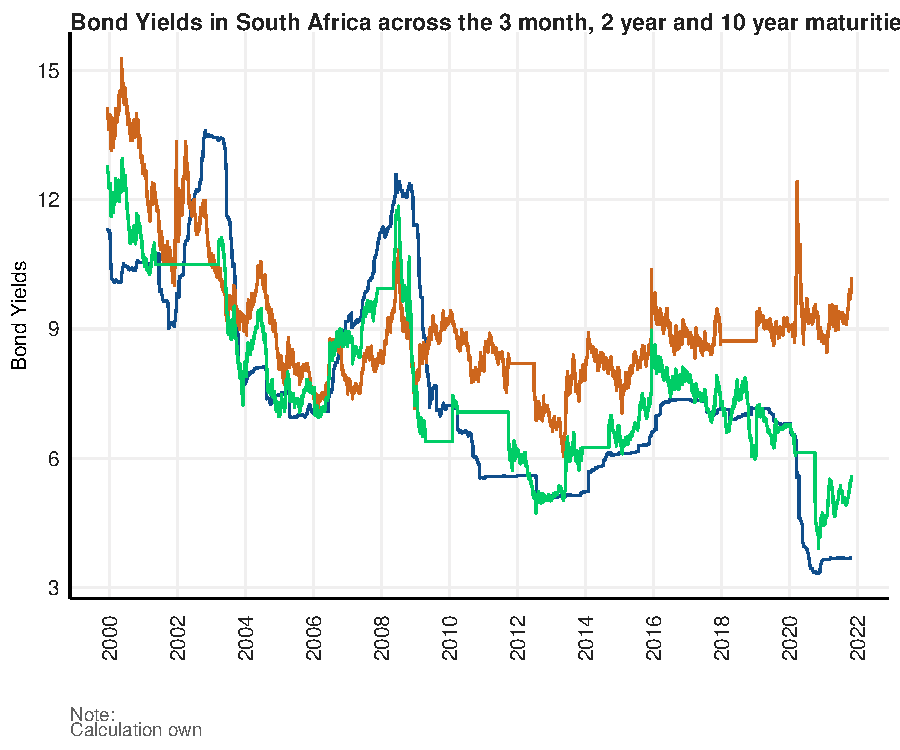
\includegraphics{Question2_files/figure-latex/unnamed-chunk-3-1.pdf}

This graph shows that over the last 20+ years bond yields have actually
decreased relatively. With the largest decline that of the shortest
maturity bond, the 3-month bond. What we can see in this graph is that
the bond yields before 2020 were moving with one another. Since 2020 you
can see a divergence of the Bond Yields, taking us to our next analysis:
Yield Spreads.

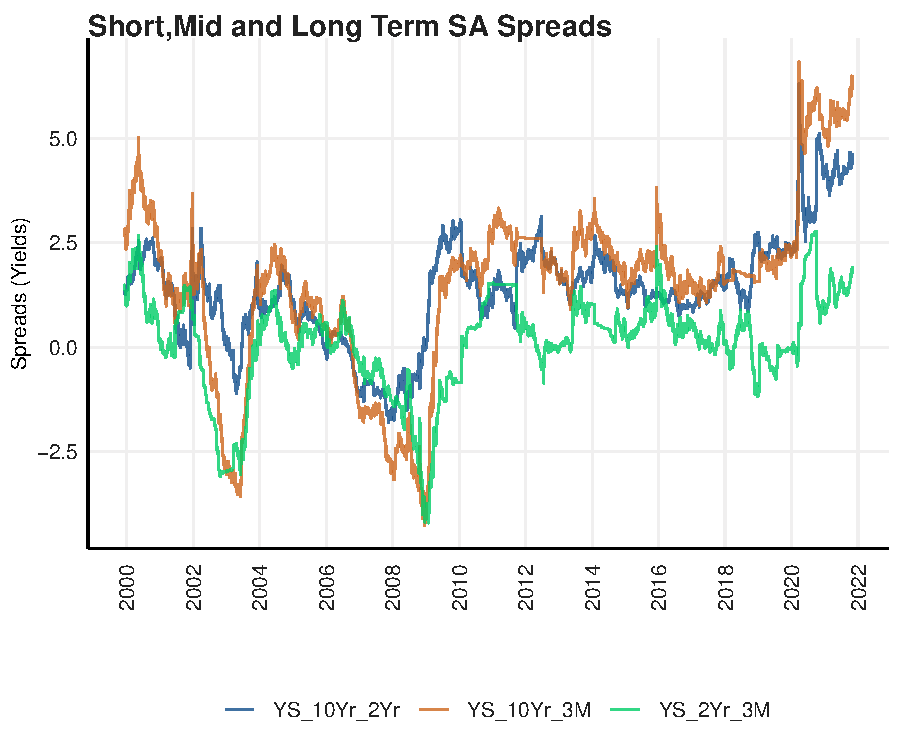
\includegraphics{Question2_files/figure-latex/unnamed-chunk-5-1.pdf}

The second plot shows that current yield spreads are higher than the
historical yield spreads. The spread between the 10-year and 3 month
bonds are the greatest, followed by the difference between the 10 year
and 2 year, and then the 2 year and 3 month. As shown in the first plot,
the 10-year yield spiked upwards, while the 3-month and 2-year fall
dramatically downwards. This plot also confirms that the spreads faced a
significant spike in 2020.

A zoomed-in look can be seen in the third plot below.

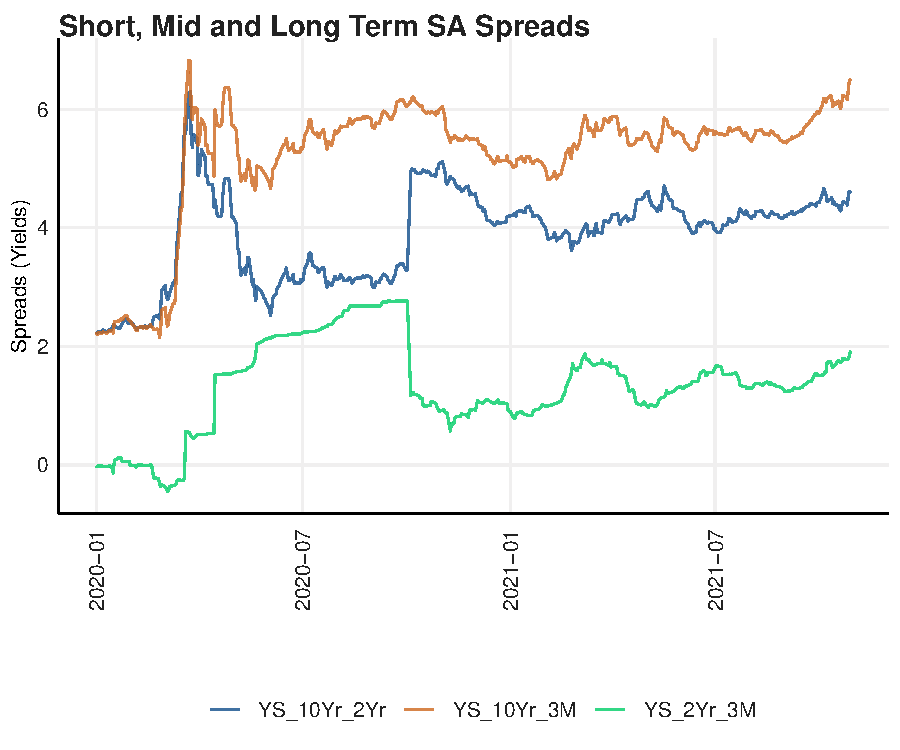
\includegraphics{Question2_files/figure-latex/unnamed-chunk-7-1.pdf}

\hypertarget{inflation}{%
\section{Inflation}\label{inflation}}

Here we look at the relationship between South African Inflation and the
Break-even inflation. This relationship can be observed in the figure
below.

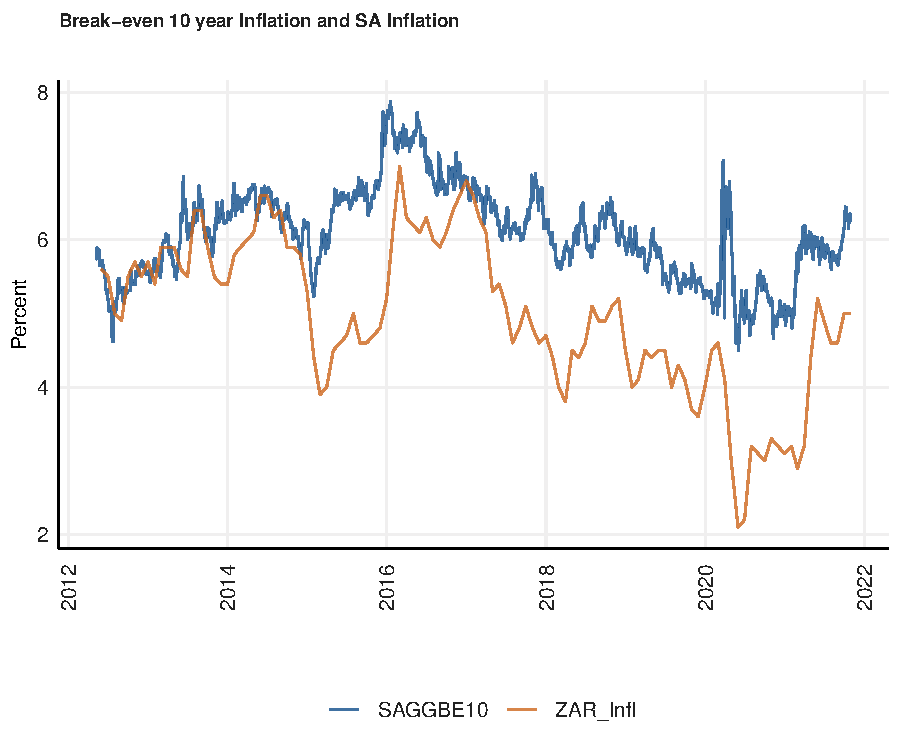
\includegraphics{Question2_files/figure-latex/unnamed-chunk-9-1.pdf}

Break-even Inflation is the difference between the nominal yield on a
fixed-rate investment and the real yield on an inflation-linked
investment.

If inflation averages more than the break-even, the inflation-linked
investment will outperform the fixed-rate. Conversely, if inflation
averages below the break-even, the fixed-rate will outperform the
inflation-linked. What we can see from the graph above is that since
2015 inflation has deviated from the break-even inflation with a large
gap forming in 2020. Which shows that in South Africa, the market
expectations for inflation are much higher than actual inflation. The
break-even inflation has increased steadily from 2020 which shows market
expectations of high inflation.

\hypertarget{international-sentiment}{%
\section{International Sentiment}\label{international-sentiment}}

\hypertarget{usd-zar-exchange-rate-and-bond-yields}{%
\subsection{USD-ZAR Exchange rate and Bond
yields}\label{usd-zar-exchange-rate-and-bond-yields}}

The below graph shows how the USD-ZAR exchange rate and the short,
medium and long-term bond yields moved in sync at the beginning of 2020.
The exchange rate lowered from its peak in 2020 while the long-term bond
yields remained at their high level.

Below is the Historical plot of Bond spreads and the USD-ZAR exchange
rate. What is noticeable is that before 2010 the yield spreads move in
opposite direction to the exchange rate. This changes after 2010 as we
witness the exchange rate climb steadily and in 2020 the exchange rate
and yield spreads move together.

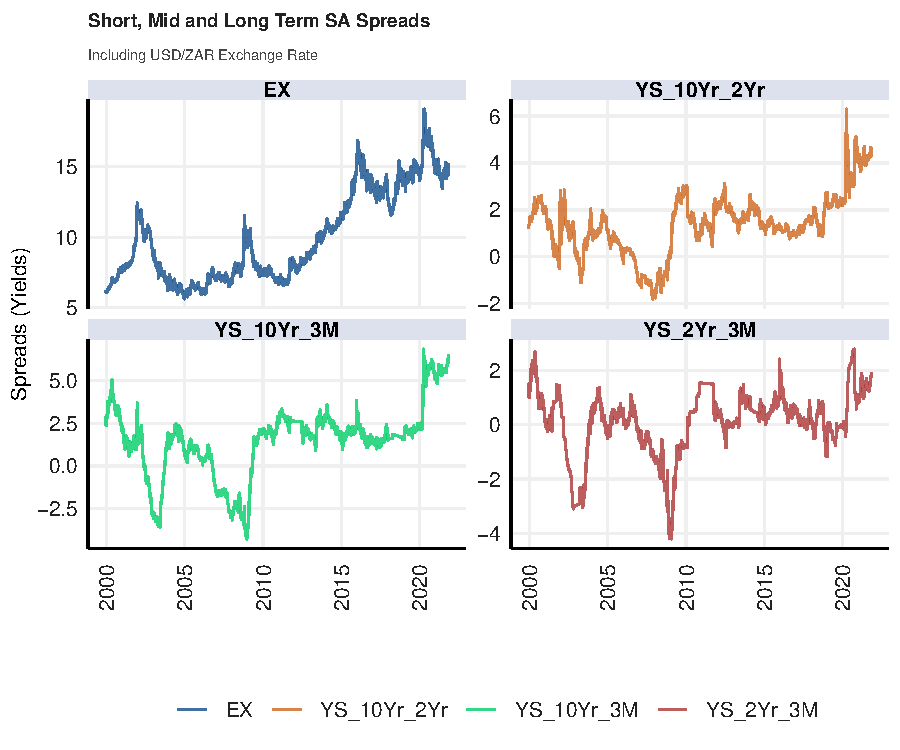
\includegraphics{Question2_files/figure-latex/unnamed-chunk-11-1.pdf}

\hypertarget{volatility-indices-and-sa-yield-spread-graph}{%
\subsection{Volatility Indices and SA Yield Spread
Graph}\label{volatility-indices-and-sa-yield-spread-graph}}

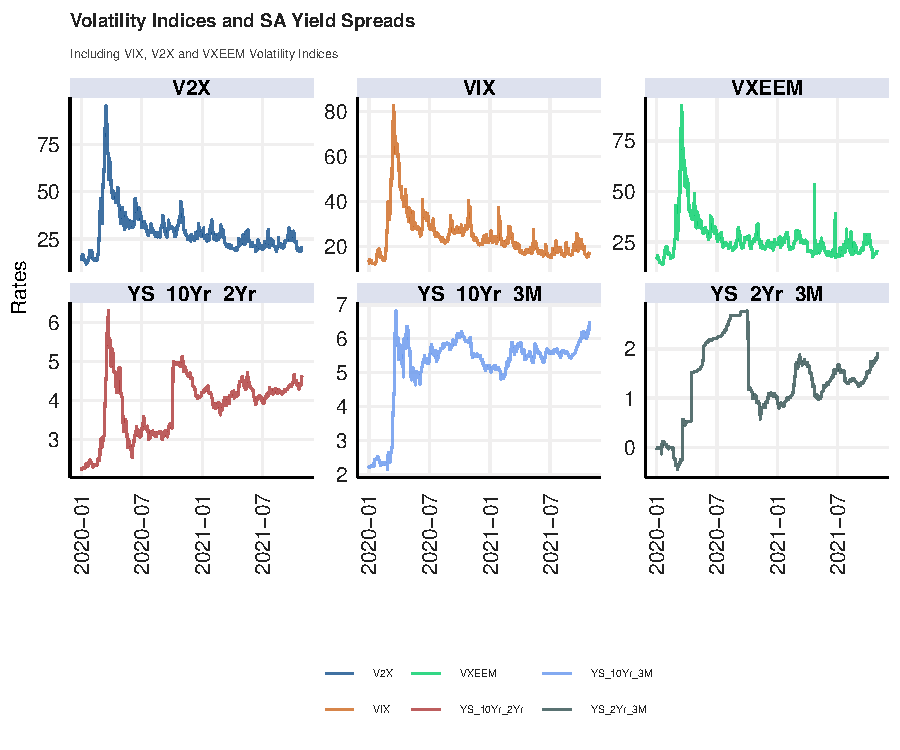
\includegraphics{Question2_files/figure-latex/unnamed-chunk-13-1.pdf}

We can see that the spike in the VIX caused a shift in all the yield
spreads. To further put this into context we will graph the 10-year to
2-year yield spread of RSA and international countries in order to see
the links between yield spreads and the VIX.

\hypertarget{foreign-yields-and-vix}{%
\subsection{Foreign Yields and VIX}\label{foreign-yields-and-vix}}

We then look to a comparison of long-term yield spreads across different
countries with the volatility index as a reference point. Below is a
graph of the 10-year to 2-year yield spreads for South Africa, the
United Kingdom and the Unites States. We can see below that all of the
yield spreads initially spike with the VIX but the yield spreads for SA
has the largest spike, with the UK next and the US last. This confirms
that global risk sentiment, movement out of emerging market bonds and
into safer developed markets bond was a contributing factor to higher
yields in South Africa during the onset of COVID-19 in 2020.

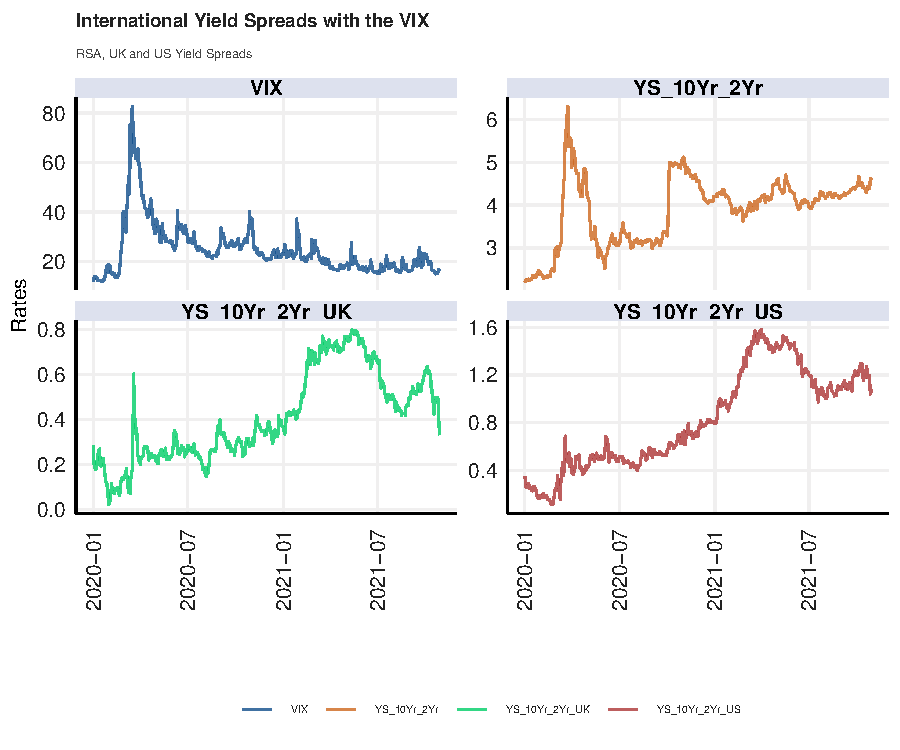
\includegraphics{Question2_files/figure-latex/unnamed-chunk-15-1.pdf}

\hypertarget{conclusion}{%
\section{Conclusion}\label{conclusion}}

Capital outflows into safer developed market bonds caused the demand for
South African bonds to decrease, and therefore their yields to increase.
The SARB adopted a mild form quantitative easing for the first time
which kept the 3-month and 2-year yields low. However, the 10-year yield
increased, and in turn its spread with bonds of shorter maturity. Thus I
do agree with the initial hypothesis that the yield spreads are greater
than historical norms.

\bibliography{Tex/ref}





\end{document}
